\section{Biohazard}

\subsection{Introducci\'on}
Este problema trata sobre transportar una cantidad  $n$ de productos químicos en camiones especiales para su traslado, sabemos que cada par de productos $p_{i}$ y $p_{j}$ reaccionan de distinta forma y por eso tiene un coeficiente de peligrosidad denominado $h_{ij}$. \\
Por normas de seguridad el nivel de peligrosidad de los productos transportados en un camión no puede superar un valor $M$, dicho nivel se mide de la siguiente manera:

$h(P) = \sum\limits_{\substack{
p_{i},p_{j} \epsilon P \\
i<j}} h_{ij}$ 


Nuestro objetivo es indicar como distribuir los productos químicos en los distintos camiones de forma de utilizar la menor cantidad de camiones posibles. \\ \\

A continuación un ejemplo del problema con su solución:


\begin{figure}[H]
  \centering
	\begin{subfigure}[b]{0.3\textwidth}
	
\begin{tabular}{| l | l |}
\hline
Cantidad de químicos:   & 2 \\ \hline
M:  & 20 \\ \hline
\end{tabular}


\begin{tabular}{| l | l | l |}
    \hline
    Peligrosidad Quimicos & 1 & 2 \\ \hline
    1 & 0 & 7 \\ \hline
    2 & 7 & 0 \\ \hline
\end{tabular}

	\end{subfigure} 
	\begin{subfigure}[b]{0.8\textwidth}

	 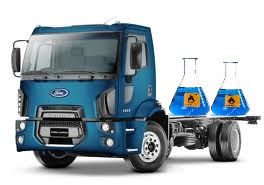
\includegraphics[scale=0.9]{Imagenes/Ej3/intro}
      
     \end{subfigure}
     \caption{Para este ejemplo los dos quimicos entran en 1 camion}
\end{figure}

\subsection{Desarrollo}


Para la resolución de este problema se no pidió que usáramos la técnica de Backtracking, por lo que nuestra idea del algoritmo comenzó por ir probando para cada producto químico todas las posibilidades de guardarlo en $n$ camiones (ya que como mucho metemos cada producto en un camión distinto), es decir la posibilidad de meter el químico $i$ al camión 1 y el resto de los químicos en distintos camiones, la posibilidad de meter los químicos $i$ y $j$ con $i$ != $j$ en el camión 1 y el resto en otros camiones, etc. Eventualmente nos quedamos con la posibilidad generada en la cual se usan menos camiones y no se supere el umbral $M$. \\
Luego pensamos podas y estrategias para mejorar al algoritmo, se nos ocurrieron las siguientes: 

\begin{itemize}
	\item Si probamos todas las posibilidades de distribuir los químicos en los distintos camiones con los químicos $i$ y $j$ con $i$ != $j$ en el camión 1, no vamos a probar lo mismo para el camión 2. Es decir, elimina todas las permutaciones en otros camiones de la misma solucion. \\
	Esta poda es buena en los casos donde hay muchos químicos que transportar pues entre más químicos hay, mas ramas de soluciones aparecen.
	
	\item Si en una rama del algoritmo tenemos un camión donde ya metimos $x$ productos químicos y al agregar un nuevo producto supera el umbral, entonces descartamos esa posibilidad. \\
	Esta estrategia es algo básica pero permite descartar ramas innecesarias las cuales no conducirán a una solución para el problema
 
\end{itemize}


\subsubsection{Pseudocódigo}

\LinesNumbered
\begin{algorithm}[H]
\DontPrintSemicolon
\KwData{\textbf{camiones}: conjunto de camiones, \textbf{productos}: conjunto de sustancias, \textbf{solucion}: conjunto de camiones}
\Begin{
	contador $\Leftarrow$ contar(camiones)\;
	\If{contador $ < $ minimosCamionesUsados} {

		\If{productos.todosUsados()} {
			minimosCamionesUsados $\Leftarrow$ contador \;
			solucion $\Leftarrow$ camiones \;
		}
		\For{ sust $\in$ productos } {
			\If{ $\not$ sust.usado() }  {
				\For{camion $\in$ camiones} {
					\If {(camion.noEsPeligroso(umbral, sust))} {
						camion.agregarSustancia(sust)\;
						Biohazard(camiones, productos, solucion)\;
						camion.sacarSustancia(sust)\;
					}
				}
			}
		}
	}
}
\caption{\textbf{Biohazard } \label{Biohazard }}
\end{algorithm}

La función contar, cuanta la cantidad de camiones utilizados. 
La función noEsPeligroso determina si agregar la sustancia al camión no supera el umbral.


\subsection{Complejidad}
Analicemos primero la naturaleza del problema. Tenemos n productos químicos los cuales tenemos que enviarlos a una fábrica mediante camiones. Nuestro objetivo es minimizar la cantidad de camiones contratados. Entonces podemos pensar un primer acercamiento en el cual comenzamos con n camiones. Esta va a ser nuestra solucion trivial, un camion por producto. A continuación probamos todas las maneras de distribuir los productos en estos camiones de manera tal que la cantidad de camiones contratados sea minima. Algo a resaltar es que un producto x pertenece a un camión nada mas (los productos son distinguibles). Entonces, cuantas maneras de distribuirlos tenemos?

Tenemos los productos $p_{1}$ $p_{2}$ y $p_{3}$. Pensemos esto como anagramas donde cada producto y camion es una letra. Sea $p_{i}$ la letra asociada al producto i y | la letra asociada al camion. Entonces lo que queremos buscar son la cantidad de anagramas que podemos formar con las letras $p_{1}$|$p_{2}$|$p_{3}$ en donde el orden de los camiones no nos importa. Si n = \# productos y m= \# camiones la formula sería:

$\frac{(n+m-1)!}{(m-1)!}$

En nuestro caso, m = n quedando

$\frac{(2n-1)!}{(n-1)!}$

Claramente la complejidad es exponencial.

Esta versión es nuestro algoritmo de backtracking sin ninguna poda. Ahora bien, algo importante a notar es lo siguiente: supongamos que tenemos 5 productos, y la distribucion optima es poner el producto $p_{1}$ $p_{2}$ y $p_{3}$ en un camion y el producto $p_{4}$ y $p_{5}$ en otro. Como nosotros partimos de tener n posibles camiones (en este caso serían 5), se solaparian las distribuciones donde $p_{1}$ $p_{2}$ y $p_{3}$ estan en el camion 1 mientras que los productos $p_{4}$ y $p_{5}$ en el camion 2 con las que esten $p_{1}$ $p_{2}$ y $p_{3}$ en el camion 2 con $p_{4}$ y $p_{5}$ en el camion 3. Entonces un segundo acercamiento sería sacar "`todas las permutaciones"' posibles de una distribucion dada (poda ya descripta). Esto sería lo mismo que contar los posibles subconjuntos de un conjunto cuyos elementos son los productos. Es decir, a nuestro caso $\{p_{1}, p_{2}\} = \{p_{2}, p_{1}\}$ quedando una complejidad de $O(2^n)$.

\subsection{Testing}

Decidimos tomar las siguientes instancias del problema para corroborar los resultados:\\

\textbf{Caso 1:} 2 productos químicos y el límite de peligrosidad 2. $h_{1,2}$ es 1.\\
\indent En este caso es obvio que ambos productos pueden viajar en 1 solo camión.

\textbf{Caso 2:} 3 productos químicos y el límite de peligrosidad 6. $h_{1,2} = 6, h_{1,3} = 7, h_{2,3} = 8$ .\\
\indent En un sólo camión no entran los 3 productos (tendría peligrosidad 21). Puedo poner el producto 1 y 2 en un camión, mientras que el 3 en otro camión. El mínimo en este caso es 2.

\textbf{Caso 3:} 3 productos químicos y el límite de peligrosidad 6. $h_{1,2} = 7, h_{1,3} = 7, h_{2,3} = 8$ .\\
\indent En este caso se puede ver que cada producto debe ir en camiones separados ya que la peligrosidad de a pares siempre supera el límite. En este caso el mínimo es 3.

\textbf{Caso 4:} 3 productos químicos y el límite de peligrosidad 8. $h_{1,2} = 2, h_{1,3} = 3, h_{2,3} = 3$ .\\
\indent En este caso se puede ver que todos los productos pueden viajar en un solo camión ya que la suma de sus peligrosidades es 8 y no supera el límite, que también es 8.\\

Estos casos de pruebas pueden encontrarse en \textbf{ej3/tester.cpp}.

\subsection{Experimentación}

Para los experimentos de medici\'on de tiempos decidimos armar un lote de entradas aleatorias, para generar dichas entradas, se utilizo un script en python al cual se le pasaban como par\'ametros los datos del problema y devolv\'ia valores pseudo-aleatorios.
A continuaci\'on haremos una comparaci\'on a nivel tiempo de ejecución de los algoritmos de backtracking con y sin podas, buscando confirmar que la versi\'on con podas 
tiene una mejora en el tiempo de ejecuci\'on. \\
También nos resultó interesante contrastar casos en donde la poda realizaba su mayor efecto. Comparamos (1) cuando necesitamos colocar una sustancia por camión debido a su alto indice de peligrosidad de a pares y (2) cuando podemos colocar todas las sustancias en un solo camión.

Grafico de (1)

\begin{figure}[h]
  \centering
    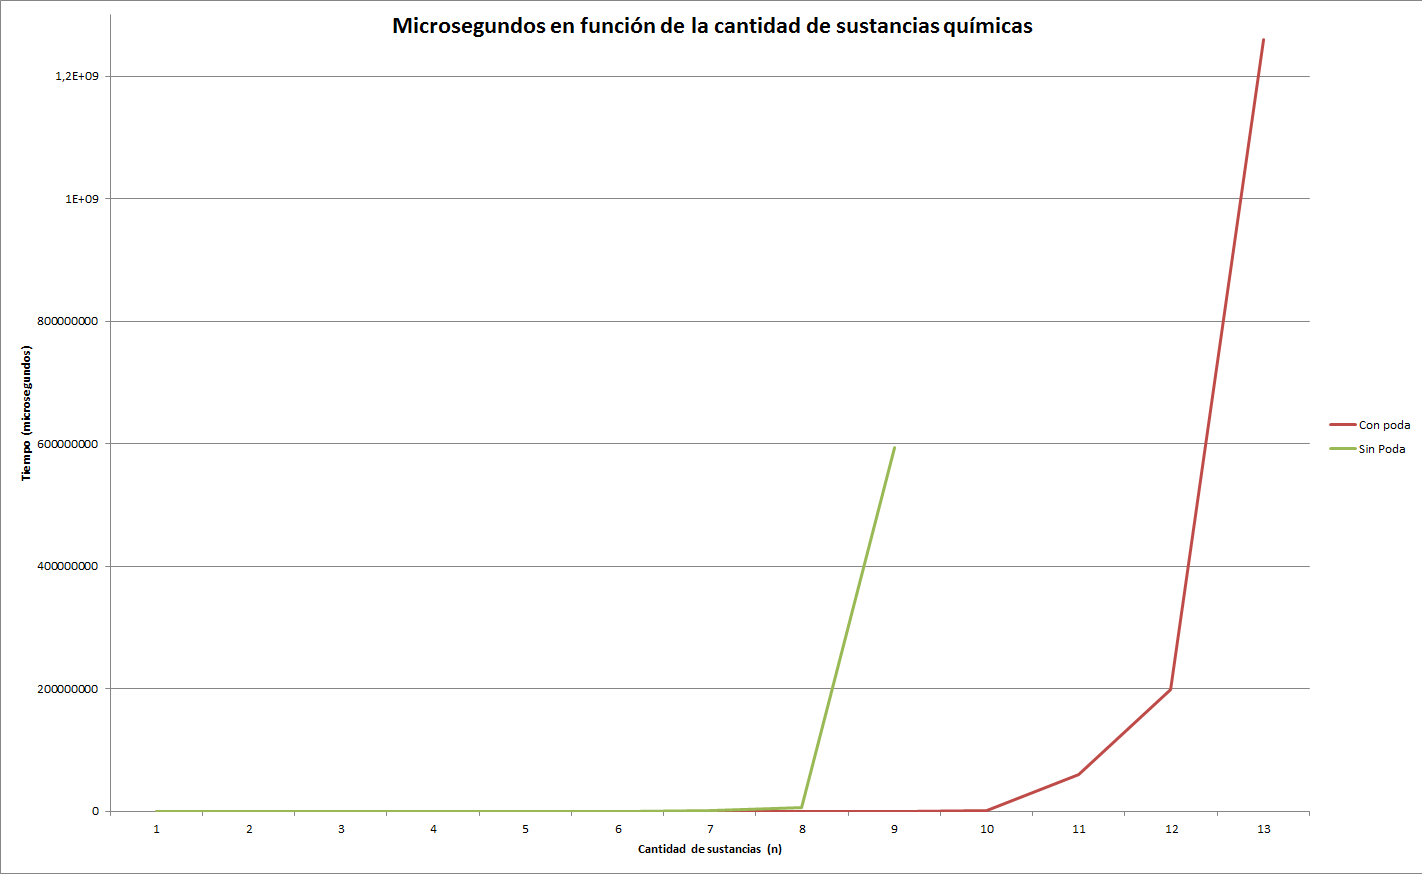
\includegraphics[scale=0.45]{Imagenes/Ej3/1solocamion.png}
  \caption{Una sustancia por camión}
  \label{fig:ejemplo}
\end{figure}

Grafico de (2)

\begin{figure}[h]
  \centering
    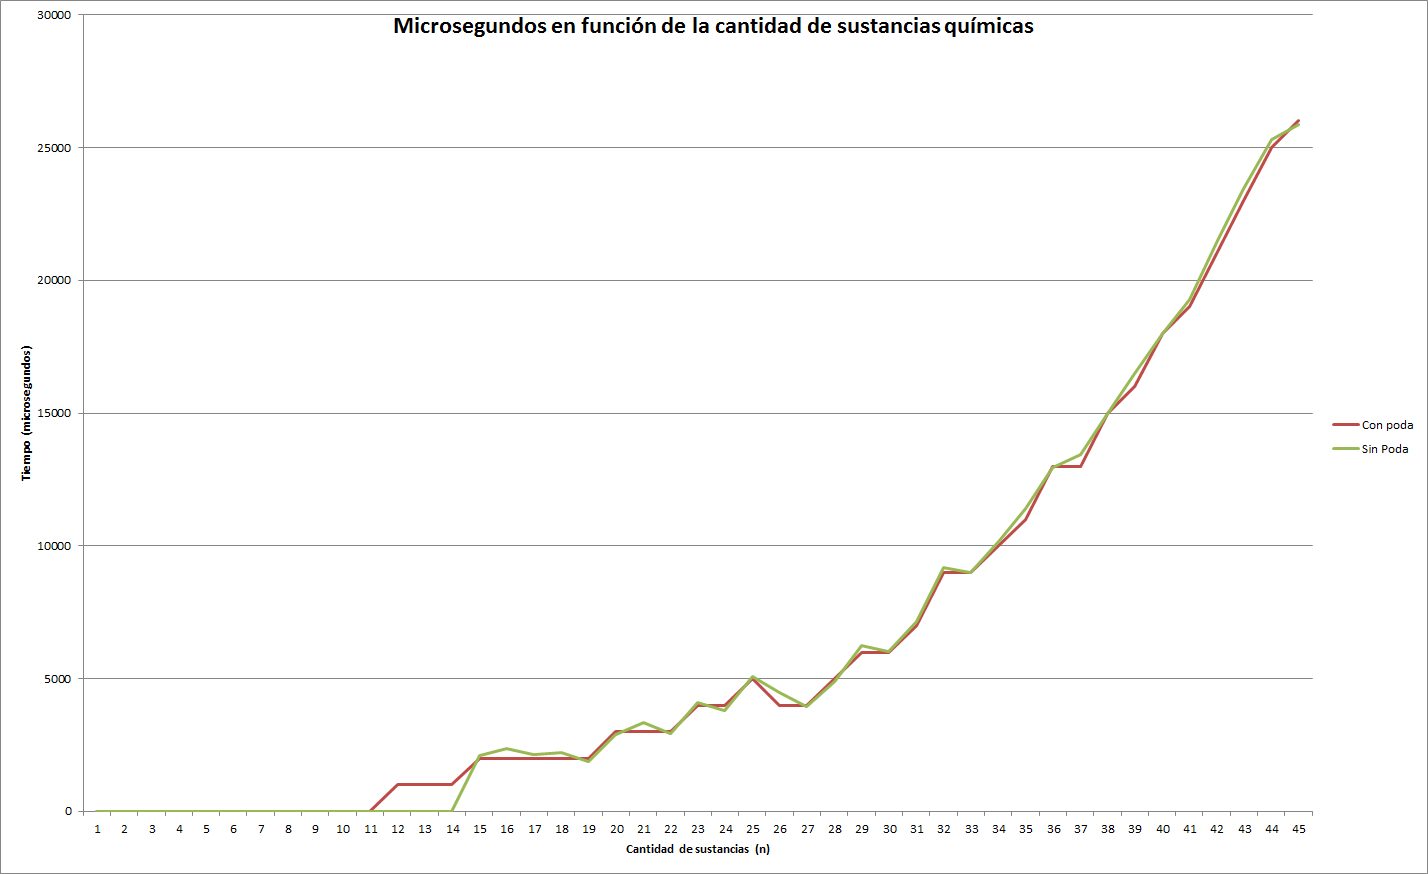
\includegraphics[scale=0.45]{Imagenes/Ej3/todo1camion.png}
  \caption{Todas las sustancias en un solo camión}
  \label{fig:ejemplo}
\end{figure}